\chapter{Analiza istniejących platform do automatyki budynkowej}
Na rynku istnieją już platformy, które są darmowe więc można stwierdzić, że zapotrzebowanie na takie platformy nie istnieje. W związku z tym można uznać, że potencjał biznesowy jest również niewielki. Systemy takie jak Home-assistant (Rys.  \ref{fig:homeAssistant}), Domoticz (Rys. \ref{fig:domoticz}) lub Node-red są darmowe oraz posiadają otwarty kod źródłowy. Warto jednak tutaj wspomnieć, że systemy te próbują na swój sposób zarabiać. Home Assistant proponuje usługę chmury gdzie użytkownik integruje swoje systemy przez panel administratora, gdzie są mu udostępniane pomocne dodatki takie jak usługa Google Assistant.
Niektóre firmy stawiają również na półdarmowe aplikacje mobilne komunikujące się z platformami, które za opłatą udostępniają na przykład widgety, które znacznie poprawiają komfort obsługi.
Twórcy platform proponują różne rozwiązania, ale skupiają się na tej samej tematyce. Analizując ich działanie można wyróżnić następujące problemy:
\begin{itemize}
    \item ograniczona ingerencja w logikę systemu,
    \item trudność z integracją urządzeń których producent platformy nie przewidział,
    \item przestarzałe technologie,
    \item toporność działania.
\end{itemize}
Poprzez różnorodność systemów użytkownicy są rozdzieleni pomiędzy tymi platformami i każdy z nich wybiera coś co spełnia jego oczekiwania.
Oprócz tego wiele komercyjnych sterowników przekaźnikowych udostępnia aplikacje mobilne do integracji produktów dla tej samej marki co jest jednocześnie głównym problemem. Takie rozwiązania proponuje Shelly, Sonoff, Xiaomi smart-home. Platformy te są również odpowiedzią dla bardzo drogich komercyjnych jednostek przeznaczonych  głównie dla domów inteligentnych działających w strukturze KNX. 
\par Tworząc platformę pewne elementy zostały zaczerpnięte z istniejących produktów, natomiast niektóre elementy mogłyby być wykonane w lepszy sposób. W tym celu podjęto próby poprawy, temat ten zostanie rozwinięty bardziej w rozdziale 4.

\begin{figure}[h]
  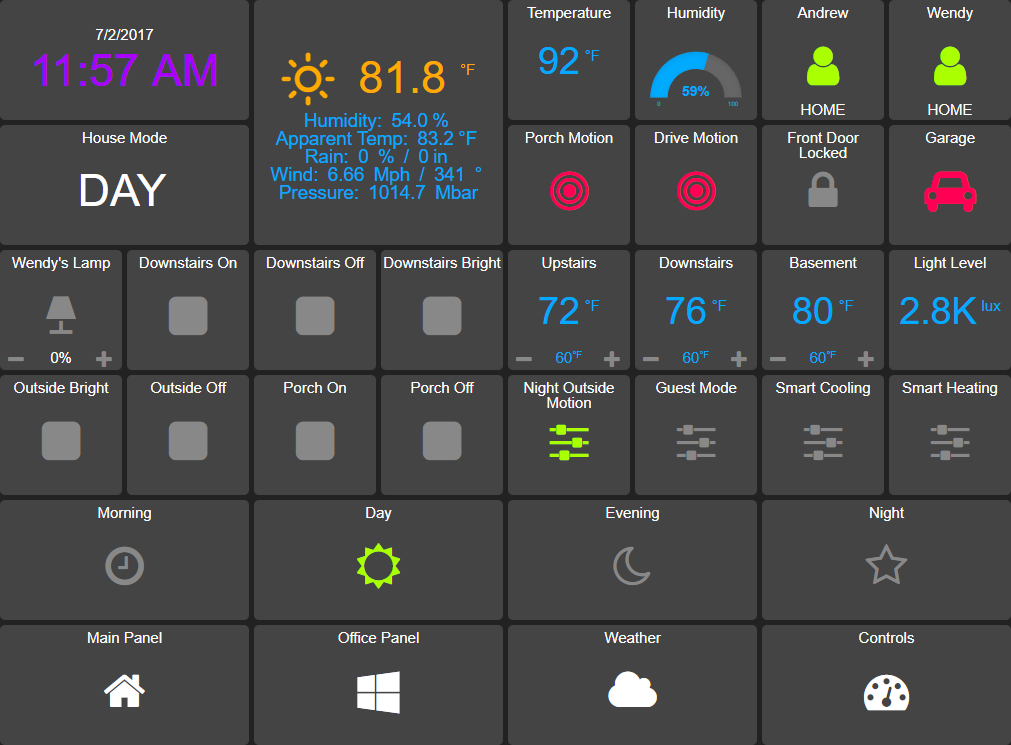
\includegraphics[width=\linewidth]{homeAssistant.png}
  \caption{HomeAssistant}
  \label{fig:homeAssistant}
\end{figure}

\begin{figure}[h]
  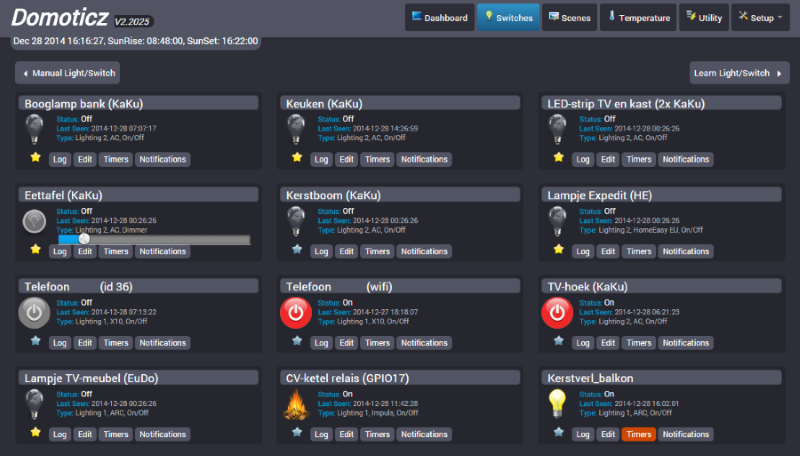
\includegraphics[width=\linewidth]{domoticz.png}
  \caption{Domoticz}
  \label{fig:domoticz}
\end{figure}